%% Template para dissertação/tese na classe UFBAthesis
%% versão 0.9.2
%% (c) 2005 Paulo G. S. Fonseca
%% (c) 2012 Antonio Terceiro
%% www.dcc.ufba.br/~terceiro/ufbathesis

\documentclass[msc, a4paper, classic, pt]{ufbathesis}
\usepackage[utf8]{inputenc}
\usepackage{graphicx}
\usepackage{url}
\usepackage{todonotes}

\newcounter{example}[section]
\newenvironment{example}[1][]{\refstepcounter{example}\par\medskip
   \noindent \textbf{Exemplo~\theexample. #1} \rmfamily}{\medskip}


%% Preâmbulo:
%% coloque aqui o seu preâmbulo LaTeX, i.e., declaração de pacotes,
%% (re)definições de macros, medidas, etc.

\title{Aplicação de um sistema fuzzy para classificação de opinião em diferentes domínios}
\date{<DATA DA DEFESA>}
\author{Matheus Cardoso de Andrade Silva}
\adviser{Prof. Dr. Angelo Loula}
\coadviser{Prof. Dr. Matheus Pires}

\begin{document}

% Folha de rosto
\dmccfrontpage{MMCC-Msc-XXXX}
% Se seu trabalho não for uma tese de doutorado do DMCC, apague a linha
% acima e use \frontpage

%%
%% Parte pré-textual
%%
\frontmatter

% Portada (apresentação)
\dmccpresentationpage
% Se seu trabalho não for uma tese de doutorado do DMCC, apague a linha
% acima e use \presenationpage

% Ficha catalográfica
\authorcitationname{<SEU NOME EM CITAÇÕES>} % e.g. Terceiro, Antonio Soares de Azevedo
\advisercitationname{<NOME DO SEU ORIENTADOR EM CITAÇÕES>} % e.g. Chavez, Christina von Flach Garcia
\coadvisercitationname{<NOME DO SEU CO-ORIENTADOR EM CITAÇÕES>} % e.g. Mendonca, Manoel Gomes de
\catalogtype{<TIPO DE TRABALHO>} % e.g. ``Tese (doutorado)''
\catalogtopics{<TOPICOS PARA FICHA CATALOGRAFICA>} % e.g. ``1. Complexidade Estrutural. 2. Engenharia de Software''
\catalogcdd{<NUMERO CDD>} % e.g. ``CDD 20.ed. XXX.YY'' (esse número vai lhe ser dado pela biblioteca)
\catalogingsheet

% Termo de aprovação - exemplo
% Modifique com os membros da sua banca
\approvalsheet{Salvador, <DIA> de <MÊS> de <ANO>}{
  \comittemember{Profa. Dra. Professora 1}{Universidade XYZ}
  \comittemember{Prof. Dr. Professor 2}{Universidade 123}
  \comittemember{Profa. Dra. Professora 3}{Universidade ABC}
  \comittemember{Prof. Dr. Professor 4}{Universidade HJKL}
  \comittemember{Profa. Dra. Professora 5}{Universidade QWERTY}
}

% Agradecimentos
% Se preferir, crie um arquivo à parte e o inclua via \include{}
\acknowledgements
<DIGITE OS AGRADECIMENTOS AQUI>

% Resumo em Português
% Se preferir, crie um arquivo à parte e o inclua via \include{}
\resumo
Opiniões são centrais em quase todas as atividades humanas, porque exercem relevante influência sobre o comportamento das pessoas. A internet e a web criaram mecanismos que tornaram possível que as pessoas pudessem compartilhar suas opiniões e para que eias, e também organizações, pudessem encontrar facilmente mais informações sobre as opiniões e experiências de outros indivíduos para ajudar em tomadas de decisão. Ainda assim, opiniões envolvem sentimentos que são descrições textuais vagas e imprecisas. Devido à natureza destes dados, a Lógica Fuzzy pode ser uma abordagem promissora para lidar com esses tipos de informações. Assim, este trabalho propõe a criação e a avaliação de sistema fuzzy para realizar um processo de mineração e classificação de opinião em diferentes domínios. Diversas características foram extraídas dos documentos e algoritmos de seleção de características foram aplicados para selecionar as mais aptas para representar e classificar os documentos. Com base nas características selecionadas, o método de Wang-Mendel (WM) e variados métodos de inferência foram utilizados para gerar as regras fuzzy e classificar documentos. Os resultados obtidos mostraram que a proposta é promissora, pois o desempenho das regras geradas se equipararam ou superaram trabalhos correlatos na literatura, demonstraram bons resultados entre domínios diferentes e ainda se igualaram a resultados de métodos clássicos de aprendizado de máquina, como o \textit{Support Vector Machine}. 
% Palavras-chave do resumo em Português
\begin{keywords}
<DIGITE AS PALAVRAS-CHAVE AQUI>
\end{keywords}

% Resumo em Inglês
% Se preferir, crie um arquivo à parte e o inclua via \include{}
\abstract
% Palavras-chave do resumo em Inglês
\begin{keywords}
<DIGITE AS PALAVRAS-CHAVE AQUI>
\end{keywords}

% Sumário
% Comente para ocultar
\tableofcontents

% Lista de figuras
% Comente para ocultar
\listoffigures

% Lista de tabelas
% Comente para ocultar
\listoftables

%%
%% Parte textual
%%
\mainmatter

% É aconselhável criar cada capítulo em um arquivo à parte, digamos
% "capitulo1.tex", "capitulo2.tex", ... "capituloN.tex" e depois
% incluí-los com:
% \include{capitulo1}
% \include{capitulo2}
% ...
% \include{capituloN}
%
% Importante: Use \xchapter ao invés de \chapter, conforme exemplo abaixo.

\xchapter{Introdução}{}

\begin{itemize}

\item Motivações
\begin{itemize}
\item As opiniões são as principais influenciadoras do comportamento humano (Liu, 2012);
\item Pessoas pedem opiniões a outras pessoas para consumo (mídia, produtos, etc.), posições políticas, religiosas, etc.;
\item Empresas precisam saber as opiniões de seus consumidores;
\item A internet e a web mudaram a forma de comunicação entre pessoas e organizações;
\item Há mais facilidade de acesso a fontes de informações e de disponibilização de opiniões (USAR DADOS PARA EMBASAR ESSA INFORMACAÇÃO);
\end{itemize}

\item Problemas
\begin{itemize}
\item Grande quantidade e diversidade de fontes de opiniões;
\item Diferentes formatos, problemas de sintaxe, gírias, dentro outros;
\item É difícil para uma pessoa comum extrair e resumir opiniões de centenas ou milhares de fontes (USAR EMBASAMENTO);
\item Opiniões são carregadas de sentimentos subjetivos e imprecisos;
\end{itemize}

\item Proposta / Definição
\begin{itemize}
\item É preciso utilizar uma metodologia para lidar com imprecisões e vagueza;
\item Lógica fuzzy (Zadeh, 1965): É uma metodologia da Inteligência Computacional que trata computacionalmente dados imprecisos e vagos;
\item ANGELO: poucos trabalhos sobre a aplicação de lógica fuzzy e/ou sistemas fuzzy foram encontrados, e os encontrados são limitados (tipo de limitação?), demonstrando uma lacuna de pesquisa sobre a aplicação de sistemas fuzzy para mineração de opiniões 
\item Por todos os problemas citadas, associadas as motivações, torna-se evidente a necessidade de sistemas automáticos de mineração de opiniões;
\item Definição de "Opinion Mining";
\item Pela vagueza das opiniões, a Lógica nebulosa pode ser útil para esses sistemas automatizados;
\item PROPOSTA: Propor e avaliar o desempenho de um sistema automatizado de mineração de opiniões baseado na lógica nebulosa;
\item DIFERENCIAL: 
\begin{itemize}
\item Geração de regras fuzzy;
\item Extração e definição de características dos documentos para geração das regras;
\item Apresentação do uso do método de Wang-Mendel no processo de mineração de opinião;
\end{itemize}

\item Perguntas de pesquisa:
\begin{itemize}
\item Como Lógica Nebulosa pode ser utilizada no processo de mineração de opiniões?
\item Quais são os ganhos, caso existam, do uso de lógica nebulosa em mineração de opiniões?
\item ANGELO: mais umas duas questões de pesquisa
\item ANGELO: depois de escrever os resultados e discussão, revisar esta seção 
\end{itemize}

\item Objetivos secundários:
\begin{itemize}
\item Investigar o estado da arte do uso de Lógica Nebulosa em mineração de opiniões;
\item Formalizar o processo de mineração de opiniões e propor uma aplicação da lógica nebulosa;
\item dentificar e compor uma base de dados para avaliação da proposta;
\item Analisar os resultados e compara-los com outros métodos da literatura;
\end{itemize}
\end{itemize}
\end{itemize}

\xchapter{Revisão da literatura}{}

\begin{itemize}
\item A área de mineração de opiniões é recente (Pang and Lee, 2008);
\item Tão recente que ainda existem problemas de terminologias (mineração de opinião, análise de sentimentos, mineração de sentimentos, análise afetiva, dentre outros);
\item Definição de opinion mining (usar um cara forte para isso, como Lib Bing, Po Pang, Turney, etc.)

\item Definição formal de opinião 'O':
\begin{itemize}
\item O = (g, s), onde \emph{g} é o alvo e \emph{s} é o sentimento associados a opinião
\end{itemize}

\item Níveis de mineração de opinião (cita e depois explica cada um deles e diz qual foi usado e por que. Além de, claro, falar de trabalhos que se encaixam em cada nível)
\begin{itemize}
\item Nível de documento;
\item Nível de sentença;
\item Nível de entidades e seus aspectos
\end{itemize}

\item Lógica Fuzzy
\begin{itemize}
\item Muitas das informações que lidamos são imprecisas e vagas;
\item A lógica clássica não consegue lidar com esse tipo de informação;
\item Para isso,Zadeh (1965) propôs a Lógica Nebulosa para lidar com informações vagas e imprecisas

\item Conjuntos Fuzzy
\begin{itemize}
\item A lógica nebulosa diz que um elemento pode fazer parte de mais de um conjunto com graus de pertinência para cada um deles (Uma opinião pode ser positiva e negativa ao mesmo tempo, mas com graus de pertinência para cada conjunto fuzzy)
\item A lógica clássica, por outro lado, determina que um objeto pertençe ou não a um conjunto (Ou uma opinião é positiva ou negativa);
\end{itemize}

\item Wang-Mendel
\begin{itemize}
\item O que é?
\item Explicar o método
\end{itemize}

\item Fala de outros algoritmos de classificação e agrupamento? Tem isso na qualificação, mas não sei se é mais pertinente (??????)

\item Métodos de classificação com uso de regras
\begin{itemize}
\item CFRM
\item GFRM
\end{itemize}
\end{itemize}
\item Trabalhos relacionados
\begin{itemize}
\item Papers with opinion mining? (Angelo: Acho que alguns principais, mais para contextualizar as abordagens, independente e dependente de domínio, classificação com palavras e com features)
\item Papers with both? (angelo: Sim, descrever rapidamente os encontrados e fazer contraste com a nossa proposta)
\end{itemize}

\end{itemize}

\xchapter{Metodologia}{}

O processo de mineração de opinião
\begin{itemize}

\item Preprocessing
\begin{itemize}
\item Definição
\item Reiterar o tipo de análise escolhida: Document Level Analysis
\item Datasets utilizados (Cornell e Amazon - descreve as caracteristicas de cada dataset, como quantidade, balanceamento, natureza, etc.)

\item Descrever e justificar as tarefas envolvidas:
\begin{itemize}
\item O texto é dividido em sentenças
\item POS Tagging - Brill's Tagger
\item Blocos irrealis são filtrados ou não (atualmente NÃO FILTRAM)
\item Defino quais ngrams serão extraídos
\begin{itemize}
\item Defino o uso do tipo de negação (FAR NEGATION - REFER)
\item Os verbos foram recentemente removidos do universo
\item Depois de testar, MANUALMENTE, diferentes configurações de n-grams, mantendo os demais parametros fixos, restaram adjetivos e adverbios, com unigrams, bigrams e trigrams
\end{itemize}

\item Retorna um vetor de n-grams (bag-of-words)
\item Resume o subcapitulo e finaliza falando da saída dessa fase para a próxima
\end{itemize}
\end{itemize}
\end{itemize}

O processo de mineração de opinião é comumente definido em seis etapas: a i) definição do domínio, ii) pré-processamento, iii) transformação, iv) seleção de características, v) classificação e vi) análise dos resultados \cite{moraes2012document}. Cada etapa inclui diferentes tarefas que, dado um documento na entrada do processo, seja possível classifica-lo e avaliar a classificação realizada.

\begin{figure}[h]
\caption{Etapas do processo de mineração de opinião.}
\centering
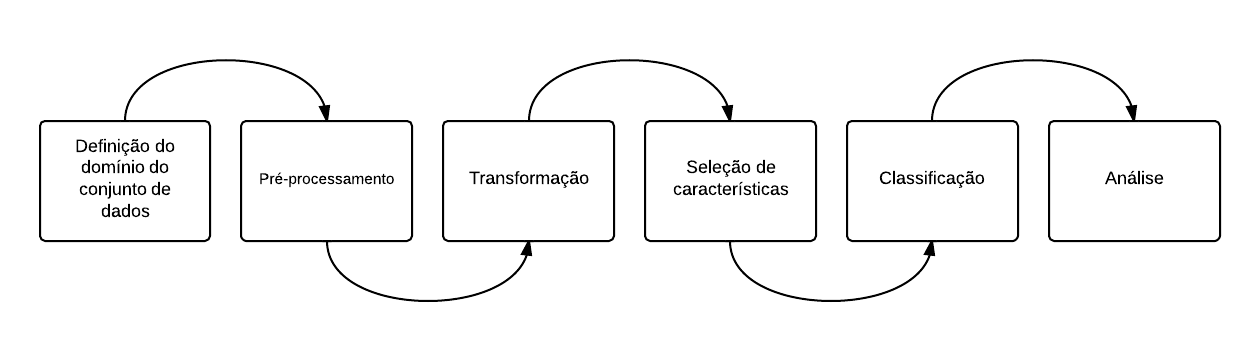
\includegraphics[scale=0.35]{opinion_mining_process.png}
\label{figura:processo_mineracao}
\end{figure}

\section{Definição do domínio e o pré-processamento dos dados}

Domínios diversos foram escolhidos para serem analisados por essa pesquisa, dentre eles filmes, livros, carros, computadores, panelas, hotéis, músicas, celulares, mp3, pen-drives, dispositivos gps, wifi e câmeras fotográficas. Essa diversidade de domínios é importante para que nós possamos corroborar nossa proposta de criar um classificador independente de domínio. Todas as bases de dados são da língua inglesa, pois os trabalhos relacionados a esta pesquisa utilizaram domínios nessa língua.

Para filmes, nós utilizamos a largamente utilizada \footnote{Vide https://www.cs.cornell.edu/people/pabo/movie-review-data/otherexperiments.html} base de dados, versão 2.0, desenvolvida e pré-classificada por \cite{pang2004sentimental}, com 2000 críticas de filmes, sendo metade positivas e outra metade negativas - bases assim, são conhecidas como balanceadas. As opiniões dos domínios de livros, carros, computadores, panelas, hotéis, músicas, celulares estão reunidos numa base de dados balanceada produzida por \cite{taboada2011lexicon}, retiradas do site Epinions \footnote{Vide http://www.epinions.com/}, com cerca de 400 críticas. E para as opiniões dos domínios de mp3, pen-drives, dispositivos gps, wifi e câmeras fotográficas, nós utilizamos uma base de dados balanceada de 2000 críticas retiradas do site da Amazon. 

Após a definição de um ou mais domínios é preciso, antes de inciar a etapa de pré-processamento, definir o nível da análise que será feita sobre os documentos. Existem três níveis básicos de análise de documentos em mineração de opinião: i) nível de análise de documento, ii) sentenças e iii) entidades e seus aspectos. O primeiro nível foca em classificar a opinião geral de um documento expressando-a como positiva ou negativa. O segundo nível, o de sentenças, em vez de considerar o sentimento geral das opiniões presentes em um documento como todo, classifica as opiniões de cada sentença separadamente. E o último nível foca em descobrir todos os alvos existentes nas sentenças do documento, e classifica as opiniões direcionadas a eles \cite{bing:2012}. Este trabalho decidiu utilizar o nível de análise de documento \cite{joachims1998text, pang2002thumbs, gamon2004sentiment, mullen2004sentiment, pang2004sentimental, cui2006comparative}.

A etapa de pré-processamento envolve tarefas como a tokenização dos documentos, marcação gramatical das palavras (do inglês, \textit{Part of Speech Tagging} ou POST), filtragem de sentenças com modais e definição os n-grams que serão utilizados para construir um modelo que represente o documento. A tokenização dos documentos é a tarefa que divide o conteúdo de cada documento em sentenças e, por sua vez, em palavras para que o marcador gramatical (ou \textit{tagger}) possa identificar as classes gramaticais das palavras do documento. O marcador gramatical usado foi o discutido em \cite{brill1995transformation} e usado em trabalhos relacionados a esta pesquisa \cite{chaovalit2005movie, taboada2008extracting, taboada2011lexicon}. A tarefa seguinte é a remoção de sentenças que possuem verbos modais. Segundo \cite{taboada2011lexicon}, modais como "would", "could", dentre outros, presentes numa sentença indicam que as palavras que aparecem juntamente com eles podem não ser confiáveis para serem usadas na definição do sentimento geral de opiniões de um documento. 

A tarefa final é definir quais n-grams serão usados para compor o modelo que representará o documento. O tipo de modelo utilizado nessa pesquisa é o popular saco de palavras (\textit{bag-of-words}), onde cada documento é representado por um vetor de termos (ou n-grams) do documento \cite{moraes2012document}. N-grams são termos que podem ser unigrams (uma palavra), bigrams (duas palavras) ou trigrams (três palavras). Nós definimos 5 tipos de n-grams: adjetivos e advérbios como unigrams; advérbios com adjetivos (e.g. \textit{very good}), advérbios com advérbios como bigrams; e a combinação de dois advérbios e um adjetivo como trigram (e.g. \textit{not very nice}) \cite{pang2002thumbs, turney2002thumbs, taboada2008extracting, karamibekr2012verb}. Nós também extraímos tipos especiais de bigrams e trigrams que são os n-grams negados (e.g. \textit{not bad}, \textit{nothing special}). A extração desses tipos de n-grams também é conhecido com detecção de negação e, por si só, é um linha de pesquisa completa, indo além do escopo deste trabalho. Nós utilizamos uma versão simplificada da técnica usada em \cite{taboada2011lexicon}. 

Ao fim do estágio de pré-processamento, cada documento é transformado num vetor de saco de palavras e é passado para a etapa de transformação. 

\section{Transformação}

\section{Seleção de características}

\section{Classificação}

\section{Avaliação}

\section{Design dos experimentos}

\documentclass[template.tex]{subfiles}
\begin{document}

\xchapter{Resultados obtidos}{}

Nessa seção são descritos e discutidos os experimentos realizados e os resultados obtidos desses experimentos. O objetivo é não só comparar qual cenário obtém melhor \textit{acuracia} ou TPR e TNR, mas também discutir em quais contextos os classificadores produzem melhores ou piores resultados.

%\section{Resultados experimentais}

Nós focamos em comparar os métodos de seleção de características e de inferência, variando as configurações em diferentes etapas do processo de mineração de opinião, comparando acurácia, TPR e TNR. Nós avaliamos a influência dos algoritmos de seleção de características, os sistemas de inferência fuzzy em si, o uso de pesos na regras, a quantidade usada de conjuntos fuzzy, a eficiência das regras entre domínios e usadas em outro,características mais selecionadas entre as bases utilizadas. 

%\todo[inline]{usa folds ao inves de dobras, já troquei no parágrafo abaixo e refiz redação também}
%\todo[inline]{matheus: ok}

%\todo[inline]{matheus: esse paragrafo ja tem na metodologia. Daí eu eliminei e juntei com o paragrafo do inicio do capitulo e eliminei essa seção também. O texto eliminado está comentádo no latex.}
%Para cada base de dados, o processo de mineração de opinião é idêntico para as etapas de pré-processamento, transformação e extração de características. Aplicando validação cruzada de 10 folds, as 9 partes da base são utilizadas para treinamento são utilizadas para seleção de características, na modelagem dos conjuntos fuzzy e na construção da base de regras fuzzy. A parte restante é utilizada somente para teste, realizando a seleção da mesmas características escolhidas durante o treino e fornecendo os valores destas para o sistema fuzzy realizar a classificação. O mesmo processo é repetido para cada fold e os resultados, para todas as medidas usadas, são a média dos valores obtidos em cada fold de teste. 

%\todo[inline]{falta mais discussão nas seções seguintes, apresente mais informações sobre o que ocorreu, e discuta os resultados a luz do comportamento do sistema}

Nossos resultados são fruto de diversos experimentos nas duas bases de dados, filmes e Amazon, com variadas combinações de configurações experimentais entre os algoritmos de seleção de características, os tipos sistemas de inferência fuzzy (utilizando pesos na regras ou não) e a quantidade usada de conjuntos fuzzy para modelar as variáveis de entrada. 

O método de seleção de características pelo algoritmo c4.5 foi realizado com duas variações: característricas até altura 1 e até altura 2 da árvore. Deixando o algoritmo construir livremente a árvore do decisão para a seleção de características, em dois cenários diferentes, nós escolhemos utilizar as características que estavam nos nós das árvores até altura 1 e 2. Isso resultou na mudança da quantidade de características selecionadas nos dois cenários. Fizemos isso para analisar também em quanto a altura da árvore de decisão do c4.5 influenciaria nos resultados. Vale notar que fizemos até altura 3, mas as características selecionadas repetiam as mesmas para altura 2. 

As tabelas \ref{table:movies_3f} e \ref{table:movies_2f} mostram os resultados na base de filmes e as tabelas \ref{table:amazon_3f} e \ref{table:amazon_2f} na base mista da Amazon. Primeiramente vamos discutir os cenários para o uso de 3 conjuntos fuzzy para modelagem das características e depois para o uso de somente 2 conjuntos.

\todo[inline]{ está faltando o sinal de mais ou menos em TPR nessa primeira tabela e tem um 0.59 perdido no meio da tabela}
\todo[inline]{matheus: alterei. nao sabia desse $\pm$}
\begin{table}[htbp]
\begin{tabular}{ @{} c*{11}c @{} }
	\rot{CFS} & \rot{C4.5 - Altura 1} & \rot{C4.5 - Altura 2} & \rot{MRFG} & \rot{MRFG c/ Pesos} & \rot{MRFC} & \rot{MRFC c/ Pesos} & Acurácia & TNR & TPR 
\\ \hline
	X &  &  & X &  &  &  & 62.9\% $\pm$ 4.25\% & 63.1\% $\pm$ 22.46\% & 62.7\% $\pm$ 22.69\% \\ \hline
	X &  &  &  & X &  &  & 67.1\% $\pm$ 3.39\% & 72.6\% $\pm$ 8.77\% & 61.6\% $\pm$ 9.77\% \\ \hline
	X &  &  &  &  & X &  & 52.25\% $\pm$ 4.92\% & 40.3\% $\pm$ 32.94\% & 64.2\% $\pm$ 30.55\% \\ \hline
	X &  &  &  &  &  & X & 56.2\% $\pm$ 5.16\% & 55.1\% $\pm$ 19.21\% & 57.3\% $\pm$ 14.26\% \\ \hline
	 & X &  & X &  &  &  & 59.2\% $\pm$ 1.83\% & 53.8\% $\pm$ 34.96\% & 64.6\% $\pm$ 37.08\% \\ \hline
	 & X &  &  & X &  &  & 70.05\% $\pm$ 0.04 & 70.4\% $\pm$ 7.11\% & 69.7\% $\pm$ 9.81\% \\ \hline
	 & X &  &  &  & X &  & 54.4\% $\pm$ 1.72\% & 47.1\% $\pm$ 42.67\% & 61.7\% $\pm$ 43.93\% \\ \hline
	 & X &  &  &  &  & X & 69.8\% $\pm$ 4.03\% & 69.3\% $\pm$ 10.15\% & 70.3\% $\pm$ 11.73\% \\ \hline
	 &  & X & X &  &  &  & 59.65\% $\pm$ 2.42\% & 60.3\% $\pm$ 35.78\% & 0.59 $\pm$ 36.9\% \\ \hline
	 &  & X &  & X &  &  & 70\% $\pm$ 3.96\% & 70.3\% $\pm$ 7.02\% & 69.7\% $\pm$ 9.81\% \\ \hline
	 &  & X &  &  & X &  & 54.5\% $\pm$ 1.76\% & 55.6\% $\pm$ 43.49\% & 53.4\% $\pm$ 44.5\% \\ \hline
	 &  & X &  &  &  & X & 69.8\% $\pm$ 4.03\% & 69.3\% $\pm$ 10.15\% & 70.3\% $\pm$ 11.73\% \\ \hline
\end{tabular}
\caption{Resultados da base de filmes, utilizando 3 conjuntos fuzzy nas variáveis de entrada}
\label{table:movies_3f}
\end{table}
	
\begin{table}[htbp]
\begin{tabular}{ @{} c*{11}c @{} }
\rot{CFS} & \rot{C4.5 - Altura 1} & \rot{C4.5 - Altura 2} & \rot{MRFG} & \rot{MRFG c/ Pesos} & \rot{MRFC} & \rot{MRFC c/ Pesos} & Acurácia & TNR & TPR  
\\ \hline
	X &  &  & X &  &  &  & 67.35\% $\pm$ 6.36\% & 57.8\% $\pm$ 11.83\% & 76.9\% $\pm$ 11.39\% \\ \hline
	X &  &  &  & X &  &  & 68.85\% $\pm$ 6.66\% & 62.4\% $\pm$ 9.72\% & 75.3\% $\pm$ 11.61\% \\ \hline
	X &  &  &  &  & X &  & 64.4\% $\pm$ 8.12\% & 51.3\% $\pm$ 13.56\% & 77.5\% $\pm$ 13.90\% \\ \hline
	X &  &  &  &  &  & X & 67.55\% $\pm$ 6.14\% & 58.2\% $\pm$ 10.04\% & 76.9\% $\pm$ 11.51\% \\ \hline
	 & X &  & X &  &  &  & 60.05\% $\pm$ 2.37\% & 44.6\% $\pm$ 35.73\% & 75.5\% $\pm$ 34.8\% \\ \hline
	 & X &  &  & X &  &  & 70.85\% $\pm$ 3.09\% & 76.8\% $\pm$ 4.57\% & 64.9\% $\pm$ 5.5\% \\ \hline
	 & X &  &  &  & X &  & 54.25\% $\pm$ 2.82\% & 34\% $\pm$ 43.26\% & 74.5\% $\pm$ 38.82\% \\ \hline
	 & X &  &  &  &  & X & 70.55\% $\pm$ 3.12\% & 75.2\% $\pm$ 5.68\% & 65.9\% $\pm$ 6.25\% \\ \hline
	 &  & X & X &  &  &  & 61.75\% $\pm$ 4.2\% & 79.4\% $\pm$ 29.30\% & 44.1\% $\pm$ 31.92\% \\ \hline
	 &  & X &  & X &  &  & 68.85\% $\pm$ 3.27\% & 85.4\% $\pm$ 8.27\% & 52.3\% $\pm$ 12.82\% \\ \hline
	 &  & X &  &  & X &  & 60.4\% $\pm$ 5.75\% & 73.7\% $\pm$ 35.86\% & 47.1\% $\pm$ 34.22\% \\ \hline
	 &  & X &  &  &  & X & 68.15\% $\pm$ 2.84\% & 80.4\% $\pm$ 8.91\% & 55.9\% $\pm$ 12.87\% \\ \hline
\end{tabular}
\caption{Resultados da base da Amazon, utilizando 3 conjuntos fuzzy nas variáveis de entrada}
\label{table:amazon_3f}
\end{table}

\section{Avaliação com o uso de 3 conjuntos fuzzy}

\subsection{Avaliação dos algoritmos de seleção de características}

Analisando as tabelas \ref{table:movies_3f} e \ref{table:amazon_3f}, é possível perceber que, em ambos os casos, o melhor resultado do c4.5 com altura 1 e com MRFG com pesos (70.05\% de acurácia, 70.4\% de TNR e 69.7\% de TPR em filmes; e 70.85\% de acurácia, 76,8\% de TNR e 64.9\% de TPR na Amazon) é maior que o melhor resultado produzido pelo CFS com MRFG usando pesos (67.1\% de acurácia, 72,6\% de TNR, 61,6\% de TPR me filmes; e 68.85\% de acurácia, 62.4\% de TNR e 75.3\% de TPR na Amazon). \todo[inline]{qual configuração destes melhores resultados? e o TNR e TPR?} \todo[inline]{matheus:alterei} Todavia, a diferença entre eles não é significativa (Wilcoxon, $p\leq0.01$). É importante observar, contudo, que o CFS utiliza, em média, quase 6 características para produzir as regras e classificar os documentos, criando mais regras e menos legíveis. O c4.5, com altura 1, por outro lado, utiliza somente uma dentre duas características para que o classificador realize a mesma tarefa com desempenho equivalente. 

Há, no entanto, uma tendência a um comportamento mais estável do CFS em relação ao c4.5, que pode ser notado nos demais resultados do CFS que mostram desvios padrão menores em TNR e TPR,  na média, que os desvios apresentados pelo c4.5, principalmente quando não são utilizados os pesos (discutidos mais adiante). A tabela \ref{table:movie_folds} mostra um exemplo da grande variação na classificação entre os folds que resultam nos altos valores de desvio padrão. É importante frisar que os folds foram definidos por amostragem estratificada, mantendo a mesma proporção de documentos positivos e negativos do base de dados total. Assim, não há um desbalanceamento nos folds que justifique tal variação de comportamento. Por outro lado, isto pode ocorrer devido ao CFS ter uma cobertura maior do espaço de dados, já que tem mais características no sistema, diferentemente do c4.5, que depende de poucas características, não explorando outras que poderiam gerar maior estabilidade.

Em relação aos piores resultados, que apresentam acurácias entre 50\% e 55\%, somente na base de filmes eles se apresentaram com mais freqüência, excetuando um único caso na base da Amazon, no cenário com c4.5 com altura 1 e usando o MRFC sem pesos. Em todos os demais cenários, CFS com MRFC e c4.5 com altura 2 e MRFC, os resultados na base da Amazon foram acima de 60\% de acurácia. Esses resultados não são conclusivos em relação a qual abordagem do algoritmo de seleção é melhor ou pior nessas configurações, contudo pela frequencia ser maior na base de filmes, esse pode ser um indicativo de bases de filmes realmente são mais difíceis de se minerar opinião \cite{pang2002thumbs, chaovalit2005movie, whitelaw2005using}.

\todo[inline]{comenta também sobre os demais resultados inclusive os piores resultados, que forma obtidos resultados com acurácia próxima de 50 por cento. E comparando as bases foi o mesmo comportamento dos resultados ou teve padrão diferente? }
\todo[inline]{matheus: feito. logo acima.}

\begin{table}[htbp]
	\centering
    \begin{tabular}{llll}
    Fold & Acurácia & TPR & TNR \\
    0 & 55.5\% & 100\% & 10.0\% \\
    1 & 52.5\% & 5\% & 100.0\% \\
    2 & 54.5\% & 96\% & 13.0\% \\
    3 & 52\% & 98\% & 6.0\% \\
    4 & 55.5\% & 99\% & 12.0\% \\
    5 & 51.5\% & 4\% & 99.0\% \\
    6 & 54.5\% & 9\% & 100.0\% \\
    7 & 57\% & 97\% & 17.0\% \\
    8 & 56\% & 14\% & 98.0\% \\
    9 & 55\% & 95\% & 16.0\% \\
    \end{tabular}
    \caption{Problema do desbalanceamento entre TPR e TNR - base de filmes, com c4.5 e MRFC sem pesos}
    \label{table:movie_folds}
\end{table}

\todo[inline]{essa tabela dos folds individuais pode ficar muito menor em uma tabela com 10 linhas, uma por fold, e 4 colunas: fold, acurácia (e não Acurácia), TPR e TNR. Indique no título dessa tabela qual a configuração do experimento executado (método de seleção,inferencia e conjuntos)}
\todo[inline]{matheus:ok}

Dentre as características selecionadas por CFS e c4.5 duas se destacaram, sendo frequentemente selecionadas dentro dos cenários testados por ambos algoritmos. São elas:
\todo[inline]{porque colocou as caracteristicas em uma tabela? faz uma lista de itens}
\todo[inline]{matheus: ok}

\begin{itemize}
\item A diferença entre as somas positiva e negativa de adjetivos e bigrams compostos estritamente por advérbio e adjetivo;
\item E a diferença entre as somas positiva e negativa de unigrams e bigrams combinados.
\end{itemize}

Para o melhor resultado apresentado na base de filmes pelo c4.5 (com altura 1 e MRFG com pesos),
\todo[inline]{qual configuração do melhor resultado?} \todo[inline]{matheus: ok} somente essas duas características foram selecionadas para gerar a base de regras e classificar os documentos. As figuras \ref{figura:movies_dist_1} e \ref{figura:movies_dist_2} mostram a distribuição dessas características na base de filmes e as figuras \ref{figura:amazon_dist_1} e \ref{figura:amazon_dist_2} na base da Amazon. 

\todo[inline]{na figura do histograma, tenta usar tons de cinza (cinza claro e cinza médio, a intersecção deve ficar em cinza escuro) para ficar mais fácil para imprimir, e aumenta o tamanho da fonte dos valores nos eixos, titulos e legenda}

\begin{figure}[phtb]
\caption{Distribuição dos valores da característica "A diferença entre as somas positiva e negativa de adjetivos e bigrams compostos estritamente por advérbio e adjetivo" na base de filmes}
\centering
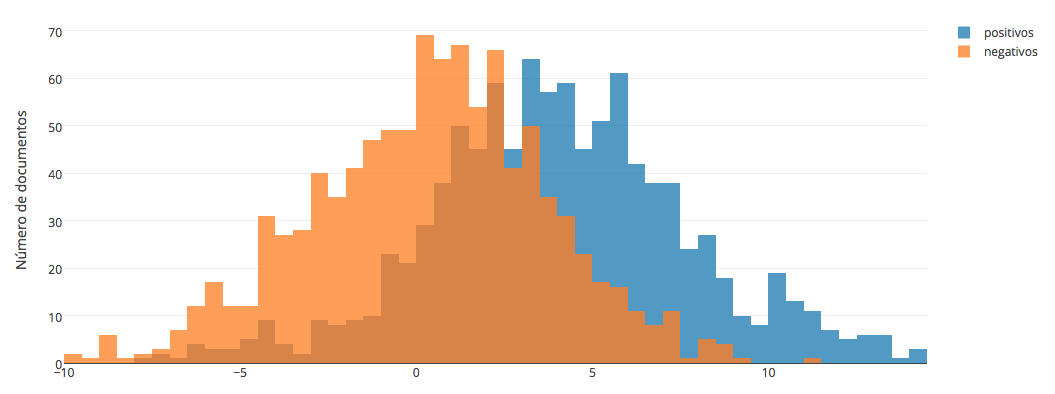
\includegraphics[scale=0.70]{movies_positive_to_negative_ratio_of_adjectives_sum_and_bigrams_with_adjectives}
\label{figura:movies_dist_1}
\end{figure}

\begin{figure}[phtb]
\caption{Distribuição dos valores da característica "A diferença entre as somas positiva e negativa de adjetivos e bigrams compostos estritamente por advérbio e adjetivo" na base de filmes}
\centering
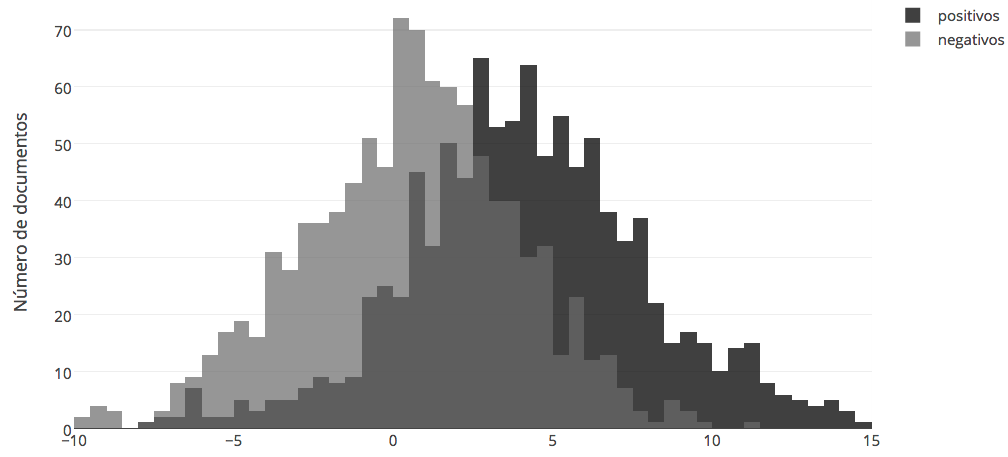
\includegraphics[scale=0.7]{movies_positive_to_negative_ratio_of_unigrams_and_bigrams_sum}
\label{figura:movies_dist_2}
\end{figure}


\begin{figure}[phtb]
\caption{Distribuição dos valores da característica "A diferença entre as somas positiva e negativa de adjetivos e bigrams compostos estritamente por advérbio e adjetivo" na base da Amazon}
\centering
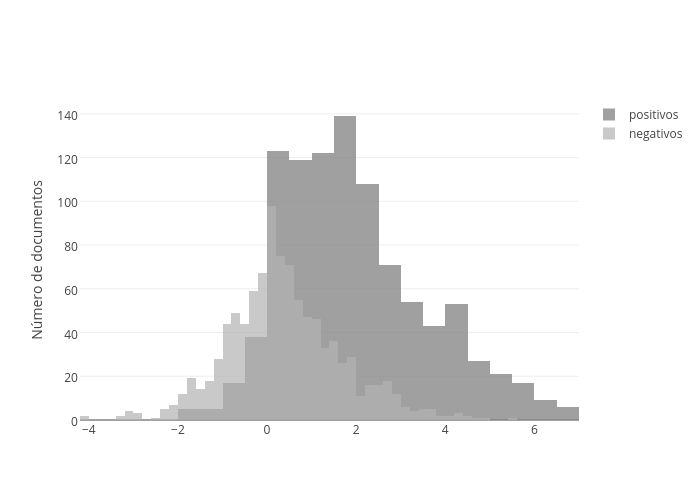
\includegraphics[scale=0.7]{amazon_positive_to_negative_ratio_of_adjectives_sum_and_bigrams_with_adjectives}
\label{figura:amazon_dist_1}
\end{figure}

\begin{figure}[phtb]
\caption{Distribuição dos valores da característica "A diferença entre as somas positiva e negativa de adjetivos e bigrams compostos estritamente por advérbio e adjetivo" na base da Amazon}
\centering
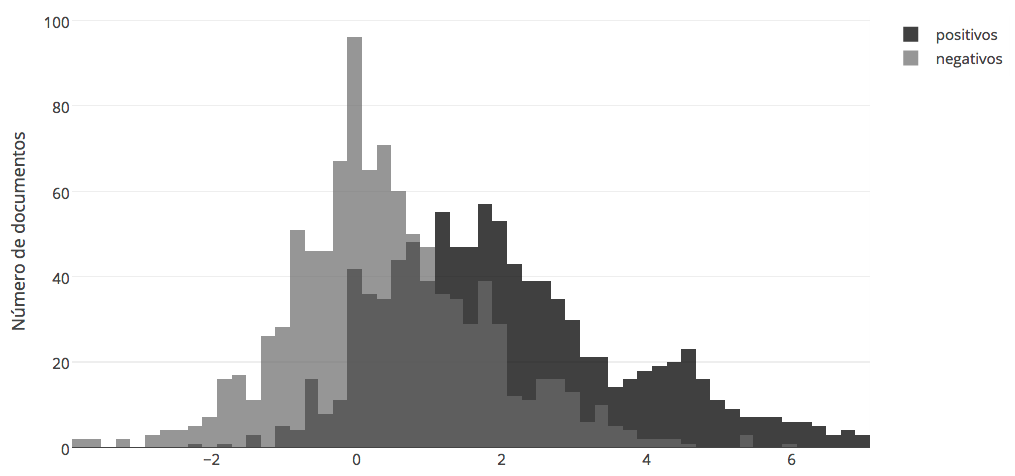
\includegraphics[scale=0.7]{amazon_positive_to_negative_ratio_of_unigrams_and_bigrams_sum}
\label{figura:amazon_dist_2}
\end{figure}

Na base de filmes, para estas características as distribuições dos documentos com polaridade positiva e dos documentos com polaridade negativa se aproximam de uma distribuição normal simétrica, enquanto na base da Amazon apresentam forte assimetria. Essa falta de equilibrio explica a mais significativa discrepância entre os valores de TPR  e TNR para o c4.5 na base da Amazon, enquanto que na base de filmes, o desequilíbrio entre essas duas medidas é menor. 
\todo[inline]{parece que a base amazon não está balanceada, a frequencia do posito está muito alta comparado com o negativo}
\todo[inline]{matheus: a base está balanceada, mas a distribuição da característica em questão é que não. Ela se apresenta mais nos positivos}

%\todo[inline]{a acurácia está péssima, quase jogar uma moeda, porque?}
%\todo[inline]{o desvio padrão aqui chamada muita atenção, está muito muito alto, , mas o cfs tem desvio menos de TNR e TPR, mas o c4.5 consegui menor desvio de acurácia, porque?}
%\todo[inline]{as caracteristicas selecionadas são sempre as mesmas? quantas diferentes? quais as mais populares? o CFS e c4.5 escolhem alguma caracteristica em comum? coloca no texto}
%\todo[inline]{pega cada tabela para discutir o que ela apresenta, TNR, TPR, acurácia, caracteristicas selecionadas, não somente descreva mas tente discutir o que ocorreu, e complemente com informações que ajudam o leitor a saber o que está ocorrendo, como informando algo sobre as caracteristicas selecionadas, as regras geradas, etc}

%SVM Filmes

%---> Avg TPR:  69.1 %
%Standard Deviation:  7.3 %
%---> Avg TNR:  72.1 %
%Standard Deviation:  6.87677249878 %
%---> Avg acuracia:  70.6 %
%Standard Deviation:  3.44818792991 %

%WILCOXON
%two-tailed

%Result 1 - Z-value
%The Z-value is -1.1212. The p-value is 0.26272. The result is not significant at p≤ 0.01.
%
%Result 2 - W-value
%The W-value is 16.5. The critical value of W for N = 10 at p≤ 0.01 is 3. Therefore, the result is not significant at p≤ 0.01.


%SVM
%
%---> Avg TPR:  65.8 %
%Standard Deviation:  4.6432747065 %
%---> Avg TNR:  75.5 %
%Standard Deviation:  3.20156211872 %
%---> Avg acuracia:  70.65 %
%Standard Deviation:  2.99207286008 %

%WILCOSOX
%
%Result 1 - Z-value
%The Z-value is -2.3953. The p-value is 0.0164. The result is not significant at p≤ 0.01.
%
%Result 2 - W-value
%The W-value is 4. The critical value of W for N = 10 at p≤ 0.01 is 3. Therefore, the result is not significant at p≤ 0.01.

%Em ambas as bases as diferenças entre os resultados não são significativas usando o teste \textit{Wilcoxon signed-rank} para $p\leq0.01$. \todo[inline]{o teste foi para acurácia? tem que dizer qual medida foi utilizada} Isso mostra que mesmo que o CFS utiliza quase 5 vezes mais características em ambas as bases e não consegue produzir resultados significativamente melhores, criando ainda regras mais complexas e de difícil compreensão para seres humanos. Assim, já que o algoritmo c4.5 somente precisou de 2 características, produzindo regras menos complexas e mais claras, para produzir resultados próximos ou iguais ao do CFS, decidiu-se em manter o c4.5 para os próximos cenários de avaliação. 
%\todo[inline]{c4.5 precisou de 2 caract? sua tabela indica 1 caracteristica, então seriam caracteristicas diferentes para cada base? ou na mesma base, folds diferentes? apresenta o histograma destas 2 caracteristicas para ilustar}

%\todo[inline]{consegue justificar porque o classificador estava jogando quase tudo para uma classe? o problema é na features selecionada, na modelagem do conjunto fuzzy, no metodo de inferencia? explica um pouco}

%\todo[inline]{ressalte que os folds foram definidos por amostragem estratificada, mantendo a mesma proporção de documentos positivos e negativos do dataset total, e assim cada fold também está balanceado, isso ajuda a mostrar que um eventual enviesamento dos folds não foi a causa deste comportamento}

%\subsubsection{Avaliação do impacto da altura da árvore de decisão do algoritmo de seleção de características do c4.5}
%\todo[inline]{acho melhor não fazer uma seção separada para arvore de altura  3, sugiro incorporar a seção anterior e incluir mais uma coluna nas tabelas, ficando c4.5 altura 1 e c4.5 altura 3}

%É importante ressaltar que os resultados anteriores, para o c4.5, foram obtidos com o algoritmo otimizado, utilizando a ferramenta Weka [CITE], para que a árvore do algoritmo de seleção de características do algoritmo tivesse altura 1, para fins de simplificação das regras geradas. Dessa forma, decidimos avaliar o quanto o aumento da altura da árvore de decisão do algoritmo de seleção de características do c4.5 influenciaria na classificação dos documentos. Definimos que o limite da altura da árvore de decisão fosse 3 para não aumentar demais a complexidade das regras que seriam geradas. A tabela (\ref{table:movies_h3}) e tabela (\ref{table:amazon_h3}) mostram, respectivamente, os resultados para este cenário nas bases de filmes e da Amazon.

%\todo[inline]{o que seria 'algoritmo otimizado'? não devemos 'forçar' a arvore a ficar com altura 3, devemos dizer que utilizamos as características  selecionadas foram aquelas existentes até altura 3, porque se a árvore crescer além disso, é só ignorar os demais nós}

% \begin{table}[!h]
%    \begin{tabular}{lll}
%    Movies                                            & c4.5 - Altura 3                                          & c4.5 - Altura 1                               \\ \hline
%    TNR                                               & 55.6\% $\pm$ 43.49\%                            & 47.1\% $\pm$ 42.67\% \\
%    TPR                                               & 53.4\% $\pm$ 44.50\%                            & 61.7\% $\pm$ 43.93\% \\
%    acuracia                                      & 54.5\% $\pm$ 1.76\%                             & 54.4\% $\pm$ 1.72\% \\
%    Características selecionadas      & 1.1 $\pm$ 0.3                                           & 1                                     \\
%    \end{tabular}
%    \caption{Resultados da base de filmes}
%    \label{table:movies_h3}
%\end{table}

%Result 1 - Z-value
%
%The Z-value is -1.7838. The p-value is 0.07508. The result is not significant at p≤ 0.01.
%
%Result 2 - W-value
%
%The W-value is 10. The critical value of W for N = 10 at p≤ 0.01 is 3. Therefore, the result is not significant at p≤ 0.01.

%\begin{table}[!h]
%    \begin{tabular}{lll}
%    Movies                                              & c4.5 - Altura 3                               & c4.5 - Altura 1                              \\ \hline
%    TNR                                                     & 73.7\% $\pm$ 35.86\%                  & 34.0\% $\pm$ 43.26\%  \\
%    TPR                                                 & 47.1\% $\pm$ 34.22\%                  & 74.5\% $\pm$ 38.82\% \\
%    acuracia                                        & 60.4\% $\pm$ 5.75\%                       & 54.25\% $\pm$ 2.82\% \\
%    Características selecionadas        & 1.9 $\pm$ 0.7                                 & 1 $\pm$                                  \\
%    \end{tabular}
%    \caption{Resultados da base da Amazon}
%    \label{table:amazon_h3}
%\end{table}

\todo[inline]{nas tabelas que mostram resultado do c4.5 altura 3, indicam um valor baixo da quant media de caract selecionadas, a mesma caracteristica está sendo selecionada por vários nós? diga quais são e discuta no texto esse comportamento, isso pode indicar que uma característica é repeditamente relevante em vários splits dos dados (cada nó da árvore de decisão, divide a base para os nós seguintes)}
\todo[inline]{matheus: ok. As características que se repetem nos nós são exatamente as duas que se destacam entre as bases}

Por fim, é válido discutir as características selecionadas usando o c4.5 com altura 2. A duas características já listadas são predominantes em quase todos os nós das árvores geradas entre os folds. Todavia, além disso, elas se repetem entre os nós das árvores, em alguns casos. É comum notar que em alguns folds a mesma característica é selecionada no nó raiz e no nó seguinte da árvore. Isso pode indicar que essas características são repetidamente relevantes em várias divisões dos dados. 

%Result 1 - Z-value
%
%The Z-value is -2.1915. The p-value is 0.02852. The result is not significant at p≤ 0.01.
%
%Result 2 - W-value
%
%The W-value is 6. The critical value of W for N = 10 at p≤ 0.01 is 3. Therefore, the result is not significant at p≤ 0.01.

%Mais uma vez, os resultados apresentados em ambas as bases para o aumento da altura da árvore de decisão do algoritmo de seleção de características não produziram resultados significativamente melhores para $p\leq0.01$ no teste \textit{Wilcoxon signed-rank}. \todo[inline]{sempre precisa dizer qual medida está sendo avalida pelo testes estatístico, reveja aqui e no restante do texto} Assim, o crescimento da árvore, que resulta no aumento da complexidade das regras em relação a altura 1, não contribui para o aumento de performance do nosso classificador e na simplificação das regras geradas para a classificação. 

\subsection{Avaliação dos sistemas de inferência fuzzy}

Após análise dos métodos de seleção de características, avaliamos agora o desempenho dos sistemas de inferência escolhidos, o Método do Raciocínio Fuzzy Geral (MRFG) e o Método do Raciocínio Fuzzy Clássico (MRFC). Os resultados mostram que em todos os cenários, independente do algoritmo de seleção usado, o MRFG produz melhores melhores percentuais de acurácia que o MRFC, mesmo que em alguns casos a diferença não seja significativa (Wilcoxon, $p\leq0.01$). Isso indica que a abordagem do MRFC de utilizar uma única regra para classificação ao invés de ponderar todas as regras , como faz o MRFG, é uma abordagem que tente a ter menos eficácia. É importante observar, contudo, que ambos os métodos apresentam altos desvios padrão nas medidas de TPR e TNR em todos os métodos de seleção, mostrando ainda instabilidade no sistema, como exemplificado na tabela \ref{table:movie_folds}, mesmo que menor. 

O uso de pesos nas regras, por outro lado, diminuiu bastante os desvios padrão de TPR e TNR, além de aumentar o desempenho geral (acurácia) do classificador em todos os cenários. Destaque principalmente para os cenários que usam o c.4.5, com menos características e, por conseguinte, menos regras, para a melhora significativa de acurácia (Wilcoxon, $p\leq0.01$) na base de filmes, usando c4.5 com altura 1 e o MRFG usando pesos, que saltou de 59,2\% (sem pesos) para 70,05\% de acurácia; e na base da Amazon, no mesmo cenário, saltando de 60,05\% para 70,85\% de acurácia. Ainda nesses cenários, os desvios padrão de TPR e TNR estavam acima de 30\% e, utilizando os pesos, caíram para menos de 10\% em filmes e 6\% na base mista da Amazon.

Isso acontece pois a aplicação dos pesos aumenta o espaço de cobertura das regras mais relevantes (ou com capacidade maior de classificar mais e melhor documentos) e diminui o espaço de regras que não tem a mesma importância e que são capazes de classificar somente uma menor região do espaço de dados. Por exemplo, as regras a seguir foram geradas um alguns dos folds para classificação usando c4.5 na base de filmes:

\begin{itemize}
\item Fold 0
\begin{itemize}
\item SE a diferença entre as somas positiva e negativa de adjetivos e bigrams compostos estritamente por advérbio e adjetivo é BAIXA então a polaridade é NEGATIVA;
\item SE a diferença entre as somas positiva e negativa de adjetivos e bigrams compostos estritamente por advérbio e adjetivo é MÉDIA então a polaridade é POSITIVA;
\item SE a diferença entre as somas positiva e negativa de adjetivos e bigrams compostos estritamente por advérbio e adjetivo é ALTA então a polaridade é POSITIVA;
\end{itemize}
\item Fold 1
\begin{itemize}
\item SE a diferença entre as somas positiva e negativa de unigrams e bigrams combinados é BAIXA então a polaridade NEGATIVA;
\item SE a diferença entre as somas positiva e negativa de unigrams e bigrams combinados é MÉDIA então a polaridade NEGATIVA;
\item SE a diferença entre as somas positiva e negativa de unigrams e bigrams combinados é ALTA então a polaridade POSITIVA;
\end{itemize}
\end{itemize}

Em quase todos os folds, as regras foram as mesmas. Contudo, em cada fold, as regras tem igual importância, quando não se utiliza os pesos. O resultado da classificação usando essas (e as demais geradas) com MRFG como sistema de inferência e sem pesos é apresentado na tabela \ref{table:movie_folds_2}.

\begin{table}[htbp]
	\centering
    \begin{tabular}{llll}
    Fold & Acurácia & TPR & TNR \\
    0 & 59.0\% & 97\% & 21.0\% \\
    1 & 57.5\% & 17\% & 98.0\% \\
    2 & 60.0\% & 91\% & 29.0\% \\
    3 & 60.0\% & 98\% & 22.0\% \\
    4 & 61.0\% & 98\% & 24.0\% \\
    5 & 55.0\% & 14\% & 99.0\% \\
    6 & 58.0\% & 18\% & 98.0\% \\
    7 & 60.5\% & 94\% & 27.0\% \\
    8 & 61.5\% & 29\% & 94.0\% \\
    9 & 59.5\% & 90\% & 29.0\% \\
    \end{tabular}
        \caption{Resultados com c4.5 com algura 1 e MRFG sem pesos na base de filmes}
    \label{table:movie_folds_2}
\end{table}

\todo[inline]{essa tabela dos folds individuais pode ficar muito menor em uma tabela com 10 linhas, uma por fold, e 4 colunas: fold, acurácia (e não accuracy), TPR e TNR. Indique no título dessa tabela qual a configuração do experimento executado (método de seleção,inferencia e conjuntos)}
\todo[inline]{matheus: ok, mas que conjuntos são esses?}

É possível perceber a instabilidade do sistema e recordar a tabela \ref{table:movies_3f} que nos mostra o resultado final de 59.2\% de acurácia, 53.8\% $\pm$ 34.96\% de TNR e 64.6\% $\pm$ 37.08\%, portanto com altos valores de desvios padrão. O uso dos pesos, porém, vai alterar a importância entre as regras, dando maior relevância àquelas mais aptas à classificação. As mesmas regras acima recebem os seguintes pesos:

\begin{itemize}
\item Fold 0
\begin{itemize}
\item SE a diferença entre as somas positiva e negativa de adjetivos e bigrams compostos estritamente por advérbio e adjetivo é BAIXA então a polaridade é NEGATIVA - \textbf{Grau: 0.60801671};
\item SE a diferença entre as somas positiva e negativa de adjetivos e bigrams compostos estritamente por advérbio e adjetivo é MÉDIA então a polaridade é POSITIVA - \textbf{Grau: 0.01536631};
\item SE a diferença entre as somas positiva e negativa de adjetivos e bigrams compostos estritamente por advérbio e adjetivo é ALTA então a polaridade é POSITIVA  - \textbf{Grau: 0.6912395};
\end{itemize}
\item Fold 1
\begin{itemize}
\item SE a diferença entre as somas positiva e negativa de unigrams e bigrams combinados é BAIXA então a polaridade NEGATIVA  - \textbf{Grau: 0.49867233};
\item SE a diferença entre as somas positiva e negativa de unigrams e bigrams combinados é MÉDIA então a polaridade NEGATIVA  - \textbf{Grau: 0.01143232};
\item SE a diferença entre as somas positiva e negativa de unigrams e bigrams combinados é ALTA então a polaridade POSITIVA  - \textbf{Grau: 0.67380056};
\end{itemize}
\end{itemize}

É possível perceber que as regras do conjunto "MEDIA" recebem os menores graus, enquanto que as regras dos conjuntos "BAIXA" e "ALTA" recebem os maiores - esse comportamento se repete para todos os demais folds. Isso mostra que o conjunto "MÉDIA" e as regras relacionadas não são boas ou tão importantes para classificar os documentos usando essas características. Assim, a disputa entre as regras no momento da classificação ficará somente entre as demais. A tabela \ref{table:movie_folds_3} mostra os resultados para a mesma configuração da tabela \ref{table:movie_folds_2}, excetuando o uso dos pesos. 

\todo[inline]{o que a tabela TAL? seria table.moviefolds3? a legenda de table.moviefolds3 indica que seria sem pesos, mas acho que seria com pesos, correto?}
\todo[inline]{matheus: correto}

\begin{table}[htbp]
	\centering
    \begin{tabular}{llll}
    Fold & Acurácia & TPR & TNR \\
    0 & 71.0\% & 65\% & 77.0\% \\
    1 & 71.0\% & 65\% & 77.0\% \\
    2 & 73.5\% & 70\% & 77.0\% \\
    3 & 67.0\% & 80\% & 54.0\% \\
    4 & 75.5\% & 80\% & 71.0\% \\
    5 & 61.5\% & 50\% & 73.0\% \\
    6 & 67.0\% & 58\% & 76.0\% \\
    7 & 75.0\% & 81\% & 69.0\% \\
    8 & 69.0\% & 71\% & 67.0\% \\
    9 & 70.0\% & 77\% & 63.0\% \\
    \end{tabular}
    \caption{Resultados com c4.5 com altura 1 e MRFG com pesos na base de filmes}
    \label{table:movie_folds_3}
\end{table}

Agora, diferentemente de antes, é possível perceber a maior estabilidade do sistema e recordar a tabela \ref{table:movies_3f} que nos mostra o resultado final de 70.05\% de acurácia, 70.4\% $\pm$ 7.11\% de TNR e 69.7\% $\pm$ 9.81\%  de TPR com baixos valores nos desvios padrão.

%Da mesma maneira que foi feita na seção anterior, nós fixamos os demais parâmetros do experimento para melhor avaliar os sistemas de inferência, mantendo o algoritmo de seleção de característica c4.5 (com altura 1, para continuar buscando a geração de regras claras e de fácil leitura para humanos) e 3 conjuntos fuzzy nas variáveis de entrada. A tabela (\ref{table:movies2}) e tabela (\ref{table:amazon2}) mostram, respectivamente, os resultados para este cenário nas bases de filmes e da Amazon.
%
%\begin{table}[!h]
%    \begin{tabular}{lll}
%    ~                   & CFRM                              & GFRM \\ \hline
%    TNR                 & 47.1\% $\pm$ 42.67\%   & 53.8\% $\pm$ 34.96\%    \\
%    TPR             & 61.7\% $\pm$ 43.93\%   & 64.6\% $\pm$ 37.08\%   \\
%    acuracia        & 54.4\% $\pm$ 1.72\%       & 59.2\% $\pm$ 1.83\%    \\
%    \end{tabular}
%    \caption{Resultados dos sistemas de inferência na base de filmes}
%    \label{table:movies2}
%\end{table}

%Result 1 - Z-value
%
%The Z-value is -2.8031. The p-value is 0.00512. The result is significant at p≤ 0.01.
%
%Result 2 - W-value
%
%The W-value is 0. The critical value of W for N = 10 at p≤ 0.01 is 3. Therefore, the result is significant at p≤ 0.01.

%\begin{table}[!h]
%    \begin{tabular}{lll}
%    ~                   & CFRM                                  & GFRM \\ \hline
%    TNR                 & 34.0\% $\pm$ 43.26\%      & 44.6\% $\pm$ 35.73\%    \\
%    TPR             & 74.5\% $\pm$ 38.82\%      & 75.5\% $\pm$ 34.80\%    \\
%    acuracia        & 54.25\% $\pm$ 2.82\%      & 60.05\% $\pm$ 2.37\%   \\
%    \end{tabular}
%    \caption{Resultados dos sistemas de inferência na base da Amazon}
%    \label{table:amazon2}
%\end{table}

%Result 1 - Z-value
%
%The Z-value is -2.8031. The p-value is 0.00512. The result is significant at p≤ 0.01.
%
%Result 2 - W-value
%
%The W-value is 0. The critical value of W for N = 10 at p≤ 0.01 is 3. Therefore, the result is significant at p≤ 0.01.

%Os resultados mostram que Método Geral do Raciocínio Fuzzy (MRFG) aumenta o \textit{acuracia} sobre o MRFC, em ambas bases,  mantendo a seleção de características e a quantidade de conjuntos fuzzy inalterados. O resultado do teste \textit{Wilcoxon signed-rank} confirma a melhora significativa do MRFG sobre o MRFC, para $p\leq0.01$. Assim, nessa tarefa de classificação de somente duas classes, positivo e negativo, os resultados mostraram que uma melhor abordagem é considerar todas as regras de uma classe, em vez de uma única com maior grau. Daí, o MRFG foi a nossa escolha para prosseguir nos próximos experimentos com o fim de alcançar melhores resultados nesse trabalho.

%\subsection{Avaliação de uso de pesos nas regras dos sistemas de inferência}
%
%Em \cite{ishibuchi2001effect} foi mostrado que é possível aumentar a performance da classificação de regras fuzzy IF-THEN, aplicando pesos à elas, além do grau de compatibilidade das regras. No referido artigo, os autores descreveram o processo em que é possível melhorar o desempenho da classificação sem alterar os conjuntos fuzzy das variáveis de saída e de entrada. Baseando-se neste artigo, este trabalho calculou os pesos como se segue. Para cada regra da base de regras gerada, foi calculado o grau de compatibilidade com todos documentos do conjunto de teste. Se o documento fosse positivo, o grau de compatibilidade era acumulado em $\beta_{positivo}$; se o documento fosse negativo, o grau de compatibilidade era acumulado em $\beta_{negativo}$. Ao fim desse processo, caso ambos os betas fosse iguais, não haveria peso a ser considerado, já que as regras tem igual influência sobre o conjunto de dados que elas foram geradas. De outra forma, o peso da regra era definido pela equação \ref{eq:pesos}.
%
%\begin{equation}
%P_j = |\beta_{positivo} - \beta_{negativo}| / (\beta_{positivo} + \beta_{negativo})
%\label{eq:pesos}
%\end{equation}
%
%onde $P_j$ é o peso da regra, para $0 <= P_j <= 1$. 

%\todo[inline]{discuta qual é idéia por trás do uso de pesos, valorizar regras que de fato auxiliar a distinguir as duas classes e desvalorizar aquelas que não conseguem separar as classes}

%Uma vez que todas as regras tiveram seus pesos calculados, estes são adicionados ao processo de classificação de ambos os métodos utilizados até aqui, o MRFG e o MRFC. O peso torna-se um fator multiplicador do grau de cada regra. Assim, o MRFC em vez de somente levar em consideração a regra com maior grau de compatibilidade com o documento de teste, vai, agora, levar em consideração a regra com maior grau multiplicado pelo peso da regra. O mesmo acontece para o MRFG ao considerar o grau médio entre as classes positivo e negativo. A tabela (\ref{table:movies2_pesos}) e tabela (\ref{table:amazon2_pesos}) mostram, respectivamente, os resultados para o uso dos pesos nas bases de filmes e da Amazon usando os parâmetros até agora estabelecidos. 

%\todo[inline]{discuta mais esses resultados, há uma grande mudança qualitativa dos resultados com uso de pesos, principalmente porque o desvio padrão cai muito, quais foram as regras que ganharam pesos e quais perderam peso? quais os valores de pesos encontrados, são próximos dos valores extremos, 0 e 1? como isso ajuda a explicar os resultados ruins sem peso? discuta o desvio padrão também }

%\todo[inline]{as tabelas são para classico ou geral?}
%\begin{table}[!h]
%    \begin{tabular}{lll}
%    ~                   & S/ Pesos                              & C/ Pesos \\ \hline
%    TNR                 & 53.8\% $\pm$ 34.96\%      & 70.4\% $\pm$ 7.11\%    \\
%    TPR             & 64.6\% $\pm$ 37.08\%      & 69.7\% $\pm$ 9.81\%   \\   
%    acuracia        & 59.2\% $\pm$ 1.83\%       & 70.05\% $\pm$ 4.00\%    \\
%    \end{tabular}
%    \caption{Resultados dos sistemas de inferência na base de filmes utilizando pesos nas regras}
%    \label{table:movies2_pesos}
%\end{table}

%Result 1 - Z-value
%
%The Z-value is -2.8031. The p-value is 0.00512. The result is significant at p≤ 0.05.
%
%Result 2 - W-value
%
%The W-value is 0. The critical value of W for N = 10 at p≤ 0.05 is 8. Therefore, the result is significant at p≤ 0.05.

%\begin{table}[!h]
%    \begin{tabular}{lll}
%    ~                   & S/ Pesos                                  & C / Pesos \\ \hline
%    TNR                 & 44.6\% $\pm$ 35.73\%      & 76.80\% $\pm$ 4.57\%    \\
%    TPR             & 75.5\% $\pm$ 34.80\%      & 64.9\% $\pm$ 5.50\%    \\
%    acuracia        & 60.05\% $\pm$ 2.37\%      & 70.85\% $\pm$ 3.09\%   \\
%    \end{tabular}
%    \caption{Resultados dos sistemas de inferência na base da Amazon utilizando pesos nas regras}
%    \label{table:amazon2_pesos}
%\end{table}

%Result 1 - Z-value
%
%The Z-value is -2.8031. The p-value is 0.00512. The result is significant at p≤ 0.05.
%
%Result 2 - W-value
%
%The W-value is 0. The critical value of W for N = 10 at p≤ 0.05 is 8. Therefore, the result is significant at p≤ 0.05.

%Os resultados corroboraram as conclusões de \cite{ishibuchi2001effect} que é possível melhorar o desempenho da classificação sem alterar os conjuntos fuzzy das variáveis de saída e de entrada apenas aplicando pesos às regras geradas. O resultado do teste \textit{Wilcoxon signed-rank} também confirma a melhora significativa do MRFG usando pesos nas regras em vez de somente o grau de compatibilidade, para $p\leq0.01$.

\section{Avaliação com o uso de 2 conjuntos fuzzy}
O efeito que os pesos produziram nos sistemas de inferência, mostrou que o conjunto fuzzy "MEDIA" não estava sendo utilizado na classificação dos documentos, pois as regras geradas com esse conjunto fuzzy sempre recebiam pesos próximos de zero ou bem distantes dos pesos recebidos pelas regras que utilizavam os conjuntos "BAIXA" e "ALTA". De fato, a presença desse conjunto para a geração das regras estava influenciando negativamente nas taxas de classificação dos documentos. Assim, nós decidimos remover esse conjunto para ratificar ou não essa hipótese, além de verificar se menos regras e mais simples terão o mesmo desempenho que antes, já que um conjunto a menos na entrada significa menos regras geradas e com antecedentes menores e mais legíveis. Os resultados com dois conjuntos fuzzy na entrada podem ser vistos nas tabelas \ref{table:movies_2f} e \ref{table:amazon_2f}.

\begin{table}[htbp]
\begin{tabular}{ @{} c*{11}c @{} }
\rot{CFS} & \rot{C4.5 - Altura 1} & \rot{C4.5 - Altura 2} & \rot{MRFG} & \rot{MRFG c/ Pesos} & \rot{MRFC} & \rot{MRFC c/ Pesos} & Acurácia & TNR & TPR  
\\ \hline
	X &  &  & X &  &  &  & 68.60\% $\pm$ 7.6\% & 74.9\% $\pm$ 9.52\% & 62.3\% $\pm$ 13.84\% \\ \hline
	X &  &  &  & X &  &  & 69.05\% $\pm$ 7.59\% & 68.4\% $\pm$ 24.26\% & 69.7\% $\pm$ 13.15\% \\ \hline
	X &  &  &  &  & X &  & 66.75\% $\pm$ 7.97\% & 59.7\% $\pm$ 17.60\% & 73.8\% $\pm$ 7.79\% \\ \hline
	X &  &  &  &  &  & X & 67.5\% $\pm$ 6.73\% & 63.8\% $\pm$ 22.45\% & 71.2\% $\pm$ 12.63\% \\ \hline
	 & X &  & X &  &  &  & 70.55\% $\pm$ 3.40\% & 71.4\% $\pm$ 5.71\% & 69.7\% $\pm$ 6.03\% \\ \hline
	 & X &  &  & X &  &  & 70.9\% $\pm$ 3.07\% & 71.2\% $\pm$ 4.33\% & 70.6\% $\pm$ 3.35\% \\ \hline
	 & X &  &  &  & X &  & 70.55\% $\pm$ 3.40\% & 71.4\% $\pm$ 5.71\% & 69.7\% $\pm$ 6.03\% \\ \hline
	 & X &  &  &  &  & X & 70.9\% $\pm$ 3.07\% & 71.2\% $\pm$ 4.33\% & 70.6\% $\pm$ 3.35\% \\ \hline
	 &  & X & X &  &  &  & 70.55\% $\pm$ 3.4\% & 71.2\% $\pm$ 5.54\% & 69.9\% $\pm$ 6.04\% \\ \hline
	 &  & X &  & X &  &  & 69.65\% $\pm$ 4.12\% & 0.67 $\pm$ 12.74\% & 72.3\% $\pm$ 6.98\% \\ \hline
	 &  & X &  &  & X &  & 70.55\% $\pm$ 3.4\% & 71.4\% $\pm$ 5.71\% & 69.7\% $\pm$ 6.03\% \\ \hline
	 &  & X &  &  &  & X & 70.9\% $\pm$ 3.07\% & 71.2\% $\pm$ 4.33\% & 70.6\% $\pm$ 3.35\% \\ \hline
\end{tabular}
\caption{Resultados da base de filmes, utilizando 2 conjuntos fuzzy nas variáveis de entrada}
\label{table:movies_2f}
\end{table}

\begin{table}[htbp]
\begin{tabular}{ @{} c*{11}c @{} }
\rot{CFS} & \rot{C4.5 - Altura 1} & \rot{C4.5 - Altura 2} & \rot{MRFG} & \rot{MRFG c/ Pesos} & \rot{MRFC} & \rot{MRFC c/ Pesos} & Acurácia & TNR & TPR  
\\ \hline
	X &  &  & X &  &  &  & 71.9\% $\pm$ 3.63\% & 69.2\% $\pm$ 9.80\% & 74.6\% $\pm$ 10.49\% \\ \hline
	X &  &  &  & X &  &  & 72.4\% $\pm$ 2.36\% & 68.5\% $\pm$ 6.62\% & 76.3\% $\pm$ 7.08\% \\ \hline
	X &  &  &  &  & X &  & 70.75\% $\pm$ 2.45\% & 73.2\% $\pm$ 8.71\% & 68.3\% $\pm$ 7.62\% \\ \hline
	X &  &  &  &  &  & X & 71.5\% $\pm$ 3.04\% & 71.4\% $\pm$ 6.45\% & 71.6\% $\pm$ 7.43\% \\ \hline
	 & X &  & X &  &  &  & 70.7\% $\pm$ 3.19\% & 77.6\% $\pm$ 2.49\% & 63.8\% $\pm$ 4.99\% \\ \hline
	 & X &  &  & X &  &  & 70.8\% $\pm$ 3.27\% & 77.2\% $\pm$ 3.54\% & 64.4\% $\pm$ 3.46\% \\ \hline
	 & X &  &  &  & X &  & 70.7\% $\pm$ 3.19\% & 77.6\% $\pm$ 2.49\% & 63.8\% $\pm$ 4.99\% \\ \hline
	 & X &  &  &  &  & X & 70.8\% $\pm$ 3.27\% & 77.2\% $\pm$ 3.54\% & 64.4\% $\pm$ 3.46\% \\ \hline
	 &  & X & X &  &  &  & 68.7\% $\pm$ 3.10\% & 86.9\% $\pm$ 6.56\% & 50.5\% $\pm$ 10.40\% \\ \hline
	 &  & X &  & X &  &  & 66.9\% $\pm$ 4.12\% & 88.9\% $\pm$ 8.50\% & 44.9\% $\pm$ 15.18\% \\ \hline
	 &  & X &  &  & X &  & 71.3\% $\pm$ 2.98\% & 76.4\% $\pm$ 3.41\% & 66.2\% $\pm$ 5.6\% \\ \hline
	 &  & X &  &  &  & X & 70.85\% $\pm$ 2.68\% & 83.5\% $\pm$ 4.96\% & 58.2\% $\pm$ 5.81\% \\ \hline
\end{tabular}
\caption{Resultados da base da Amazon, utilizando 2 conjuntos fuzzy nas variáveis de entrada}
\label{table:amazon_2f}
\end{table}

\subsection{Avaliação dos algoritmos de seleção de características}

É possível observar que os melhores resultados que vimos com três conjuntos fuzzy na entrada, melhoraram um pouco, embora não tenha sido significativo (Wilcoxon, $p\leq0.01$). Na verdade, podemos notar que, diferentemente de antes, os resultados para os cenários entre c4.5 e CFS não estão tão mais distantes como antes e, na base da Amazon, os resultados obtidos utilizando o CFS superaram muitos dos resultados produzidos com o c4.5. Isso acontece, pois além do CFS selecionar mais características que cobrem mais o espaço dos dados, a regras geradas utilizam agora somente os conjuntos fuzzy que realmente tem capacidade de classificar melhor os documentos, potencializando o conjunto selecionado pelo CFS. 

Mas, a despeito da redução dos conjuntos fuzzy, a média de características selecionadas se manteve próxima a 6 nas duas bases. Além disso, as mesmas características, listadas anteriormente, que despontaram antes, se mantiveram como as mais selecionadas entre as bases e entre os métodos de seleção. Por fim, pudemos testar nossas hipóteses de que o conjunto fuzzy "MEDIA" era, de fato, descartável e que menos regras e mais simples puderam produzir resultados tão bons quanto demonstrado anteriormente com mais conjuntos fuzzy.

\subsection{Avaliação dos sistemas de inferência fuzzy}

Os resultados mostram agora que não há diferenças significativas (Wilcoxon $p\leq0.01$) em nenhum dos cenários entre os algoritmos  MRFC e MRFG. Em alguns casos, diferentemente do que ocorria antes com 3 conjuntos, o MRFC obteve, mesmo que somente numericamente, maior acurácia média que o MRFG quando utilizado o c4.5 com altura 2. Outra mudança foi a eliminação do efeito negativo do MRFC de utilizar para classificação uma única regra ao invés de analisar todo o conjunto de dados frente às regras, como é feito no MRFG. Isso pode indicar que, essa abordagem do MRFC pode ser afetada diretamente e de maneira mais expressiva pela modelagem das variáveis de entrada, enquanto que o MRFG não sofre igualmente desses efeitos. Além disso, os desvios padrão das medidas de TPR e TNR, mesmo sem utilizar os pesos nas regras, foram reduzidos significativamente, em média, para 8\% entre as bases, contra 21\% utilizando 3 conjuntos fuzzy. 

Como os pesos mostraram quais regras seriam menos relevantes e, por conseguinte, o conjunto associado, a remoção deste produziu efeitos similares nos resultados do MRFC e do MRFG sem utilizar peso algum. Os resultados melhoraram em todos os cenários, destaque para o uso com o CFS na base da Amazon, pois foram melhores significativamente (Wilcoxon $p\leq0.01$), comparando par a par com os cenários da mesma base utilizando 3 conjuntos fuzzy na entrada. 

\todo[inline]{não entendi esse parágrafo seguinte, mesmos efeito em relação a o que? surtir qual efeito? esta seção está discutindo metodo de inferencia}
\todo[inline]{matheus: era o efeito de melhorar o desempenho. FIcou ruim mesmo. Veja se melhorou}

A aplicação dos pesos utilizando 2 conjuntos, contudo, não pareceu surtir o mesmo efeito que produziu anteriormente de melhorar a acurácia final do classificador. Os resultados foram inconclusivos quanto à aplicação de pesos nestes cenários com somente 2 conjuntos fuzzy na entrada. Os cenários que utilizaram o c4.5 com altura 1 não obtiveram nenhum ganho de desempenho. Com altura 2 os pesos reduziram, inclusive, o desempenho da classificação. E nos cenários com CFS, os pesos sempre aumentaram os valores de acurácia da classificação, mesmo que não tenham sido significativos. 

%Através das últimas seções, foram mostrados resultados utilizando 3 conjuntos fuzzy para modelar nossas variáveis lingüísticas. Seguindo a nossa decisão de usar o c4.5 com altura máxima da árvore de decisão para 1 para reduzir a complexidade das regras geradas e torna-las mais legíveis para seres humanos, nós tentamos reduzir a quantidade de conjuntos fuzzy, usando somente os conjuntos "Baixo" e "Alto", para as variáveis de entrada. Esse experimento tem por fim verificar se há aumento da performance da classificação com regras mais simples e gerais. A tabela (\ref{table:movies2_pesos_2f}) e tabela (\ref{table:amazon2_pesos_2fs}) mostram, respectivamente, os resultados para o uso de somente dois conjuntos fuzzy nas variáveis de entrada nas bases de filmes e da Amazon.
%
%\begin{table}[!h]
%    \begin{tabular}{lll}
%    ~                   & 3 conjuntos fuzzy                             & 2 conjuntos fuzzy \\ \hline
%    TNR                 & 70.4\% $\pm$ 7.11\%                   & 71.2\% $\pm$ 4.33\%    \\
%    TPR             & 69.7\% $\pm$ 9.81\%                   & 70.6\% $\pm$ 3.35\%   \\
%    acuracia        & 70.05\% $\pm$ 4.00\%              & 70.9\% $\pm$ 3.07\%    \\
%    \end{tabular}
%    \caption{Resultados dos sistemas de inferência na base de filmes utilizando 2 conjuntos fuzzy na entrada}
%    \label{table:movies2_pesos_2fs}
%\end{table}
%
%\todo[inline]{parece haver um redução no desvio padrão com uso de 2 conjuntos, porque será que reduziu?}
%
%%Result 1 - Z-value
%%
%%The Z-value is -1.2741. The p-value is 0.20408. The result is not significant at p≤ 0.05.
%%
%%Result 2 - W-value
%%
%%The W-value is 15. The critical value of W for N = 10 at p≤ 0.05 is 8. Therefore, the result is not significant at p≤ 0.05.
%
%\begin{table}[!h]
%    \begin{tabular}{lll}
%    ~                   & 3 conjuntos fuzzy                             & 2 conjuntos fuzzy \\ \hline
%    TNR                 & 76.80\% $\pm$ 4.57\%              & 77.2\% $\pm$ 3.54\%    \\
%    TPR             & 64.9\% $\pm$ 5.50\%                   & 64.4\% $\pm$ 3.46\%   \\
%    acuracia        & 70.85\% $\pm$ 3.09\%              & 70.8\% $\pm$ 3.27\%    \\
%    \end{tabular}
%    \caption{Resultados dos sistemas de inferência na base da Amazon utilizando 2 conjuntos fuzzy na entrada}
%    \label{table:amazon2_pesos_2fs}
%\end{table}
%
%%Result 1 - Z-value
%%
%%The Z-value is -0.3568. The p-value is 0.71884. The result is not significant at p≤ 0.01.
%%
%%Result 2 - W-value
%%
%%The W-value is 24. The critical value of W for N = 10 at p≤ 0.01 is 3. Therefore, the result is not significant at p≤ 0.01.
%
%A tabela (\ref{table:movies2_pesos_2fs}) mostra pequena melhora na base de filmes e empate técnico na base da Amazon. Mas, estatisticamente, os resultados não são significativamente diferentes para $p <= 1$. Todavia, a redução da quantidade dos conjuntos fuzzy para as variáveis de entrada produz regras mais simples e legíveis para serem humanos. Assim, nós temos regras menos complexas com a mesma performance de regras com maior número de antecedentes. 
%
%%positive_to_negative_ratio_of_adjectives_sum_and_bigrams_with_adjectives
%%positive_to_negative_ratio_of_unigrams_and_bigrams_sum
%Em ambos conjuntos de dados somente duas características foram selecionadas pelo c4.5:
%\begin{itemize}
%\item Diferença entre a soma positiva e negativa dos adjetivos e dos bigrams formados por advérbio e adjetivo
%\item Diferença entre a soma positiva e negativa dos unigrams e bigrams
%\end{itemize}
%
%Na base de filmes as duas foram necessárias para atingir os resultados mostrados na tabela ((\ref{table:movies2_pesos_2fs})). Isso remete ao fato de documentos de filmes serem mais difíceis de ser classificados, precisando de mais características para caracterizar corretamente as opiniões \cite{turney2002thumbs, pang2004sentimental, chaovalit2005movie, ohana2009sentiment}. Já na base da Amazon, somente a segunda característica foi utilizada para classificar os documentos. Embora o algoritmo de seleção de características do c4.5 tenha decidido que somente essa característica seja suficiente, não é difícil concluir que, sendo a base da Amazon bastante diversa (e que também inclui filmes), mais características podem ser necessárias para caracterizar melhor documentos tão variados.
%Todavia, nós conseguimos classificar um pouco mais de 70\% dos documentos de filmes e da Amazon com poucas regras simples, legíveis para humanos, geradas pelo método de Wang-Mendel:
%
%\begin{itemize}
%\item IF a \textit{diferença entre a soma positiva e negativa dos unigrams e bigrams} is ALTO then POLARIDADE is POSITIVA
%\item IF a \textit{diferença entre a soma positiva e negativa dos unigrams e bigrams} is BAIXO then POLARIDADE is NEGATIVA
%\item IF a \textit{diferença entre a soma positiva e negativa dos adjetivos e dos bigrams formados por advérbio e adjetivo} is ALTO then POLARIDADE is POSITIVA
%\item IF a \textit{diferença entre a soma positiva e negativa dos adjetivos e dos bigrams formados por advérbio e adjetivo} is BAIXO then POLARIDADE is NEGATIVA
%\end{itemize}
%
%As quatro regras foram utilizadas na base de filmes e as duas primeiras regras na base da Amazon.

\section{Avaliação do uso de regras entre domínios}
\todo[inline]{faz aplicação cruzada tambem, amazon na de filmes e vice versa}
\todo[inline]{valorize mais esta seção, o resultado é MUITO interessante, mas o texto não valoriza tanto, compare com os resultados de epinions com regras amazon e filmes. Quando aplicar amazon em filmes e vice versa compare com os resultados obtidos usando as regras da própria base. O uso do classificador de uma base em outra pode indicar a existencia de regras universais e realmente independentes de domínio, mas pode haver necessidade de ajuste na modelagem dos conjuntos ou em outro aspecto talvez}
\todo[inline]{matheus: como haviamos combinado na sexta, deixaria essa avaliações cruzadas se houvesse tempo ou para o dia da defesa}

Outra avaliação que fizemos foi a validação do uso de regras entre domínios, utilizando a base inteira da Epinions como teste. Foram usadas as regras geradas da base de filmes e da base da Amazon e aplicadas à base da Epinions.
%\todo[inline]{foram usadas as regras geradas para qual fold amazon ou filmes?}
%\todo[inline]{matheus: todas. Para cada fold eu apliquei as regras na base da epinions. O resultado final é a media entre esses resultados. Coloquei no texto.}

Todas as regras de cada fold, em ambas as bases, foram utilizadas para classificar os documentos da Epinions. O resultado final é a media entre esses resultados. Para isso, a base da Epinions passou por pré-processamento, transformação e extração de características, para que as regras pudessem avaliar corretamente os documentos. É importante frisar que nenhuma adaptação foi feita às regras, ou qualquer alteração nas características selecionadas e tão pouco na modelagem dos conjuntos fuzzy para que pudesse essa avaliação entre bases pudesse funcionar corretamente. Da maneira que foram geradas na bases de filmes e Amazon, foram utilizadas na classificação dos documentos da base da Epinions. A tabela \ref{table:epinions} mostra os resultados obtidos.
%\todo[inline]{nenhuma mudança foi feita nas regras fuzzy, mas nenhuma foi feita também nas características selecionadas e na modelagem dos conjuntos, então reforça isso tambem}
%\todo[inline]{matheus: feito} 

\begin{table}[!h]
    \begin{tabular}{lll}
    ~               & Regras da Amazon                  & Regras dos Filmes \\ \hline
    TNR             & 47.05\% $\pm$ 0.35\%           & 61.7\% $\pm$ 1.41\%    \\
    TPR         & 90.5\% $\pm$ 1.11\%               & 85.8\% $\pm$ 1.22\%   \\
    acuracia    & 68.77\% $\pm$ .0.17\%             & 73.75\% $\pm$ 0.27\%    \\
    \end{tabular}
    \caption{Resultados da aplicação de regras da base de filmes e Amazon na base Epinions}
    \label{table:epinions}
\end{table}

\todo[inline]{os valores de TPR são muito mais altos que os de TNR, indicando que a classificação funcionou muito melhor para os documentos positivos, mas teve comportamento pior para os negativos, particularmente com regras da base da Amazon, isso ocorria com os dados das bases anteriores? comenta essa observação e a comparação no texto}
\todo[inline]{matheus: não consegui encontrar esse padrão entre TPR e TNR nas bases. Então eu fiz fiz a observacao sobre esse resultado e adicionei um possivel indicio de que isso pode ocorrer devido ao enviesamento natural pra o lado positivo}

Os resultados mostram que as regras geradas podem ser usadas entre domínios diferentes, produzindo resultados próximos ou melhores que os produzidos nas próprias bases, como pode ser visto na tabela \ref{table:epinions}. Além disso, os resultados também trazem a tona que foi muito mais fácil classificar documentos positivos que os negativos em ambas as bases. Embora não conclusivo, esse enviesamento para os documentos positivos pode ser um indicativo do enviesamento do uso de dicionários de opiniões que mostram uma tendência para classificar o sentimento geral de um documento para a positividade, devido a tendência natural do ser humano de utilizar linguagem positiva e evitar termos negativos \cite{boucher1969pollyanna, kennedy2006sentiment}.

\section{Comparação com classificador SVM}

\todo[inline]{esse primeiro parágrafo poderia ir para a discussão final do capítulo}
\todo[inline]{matheus: ja foi}

Realizamos uma comparação da configuração final do nosso classificador com um método clássico de aprendizado de máquina muito utilizado na tarefa de mineração de opinião, o \textit{Support Vector Machine} (SVM), e que geralmente produz bons resultados, como ser visto em \citeonline{moraes2012document}, \citeonline{pang2002thumbs}, \citeonline{pang2004sentimental} e \citeonline{wilson2004just}. 

\begin{table}[!h]
    \begin{tabular}{lll}
    ~                   & Wang-Mendel 2 conjuntos fuzzy                     & SVM \\ \hline
    TNR                 & 71.2\% $\pm$ 4.33\%                                           & 72.9\% $\pm$ 5.80\%    \\
    TPR             & 70.6\% $\pm$ 3.35\%                                       & 68.6\% $\pm$ 7.04\%   \\
    acuracia        & 70.9\% $\pm$ 3.07\%                                       & 70.75\% $\pm$ 3.70\%    \\
    \end{tabular}
    \caption{Comparação entre os resultados do método de Wang-Mendel e SVM na base de filmes}
    \label{table:movies_svm}
\end{table}

%Result 1 - Z-value
%
%The Z-value is -0.5606. The p-value is 0.57548. The result is not significant at p≤ 0.01.
%
%Result 2 - W-value
%
%The W-value is 22. The critical value of W for N = 10 at p≤ 0.01 is 3. Therefore, the result is not significant at p≤ 0.01.

\begin{table}[!h]
    \begin{tabular}{lll}
    ~                       & Wang-Mendel 2 conjuntos fuzzy                             & SVM \\ \hline
    TNR                     & 77.2\% $\pm$ 3.54\%                                               & 75.5\% $\pm$ 3.20\%    \\
    TPR                 & 64.4\% $\pm$ 3.46\%                                               & 65.8\% $\pm$ 4.64\%   \\
    acuracia           & 70.8\% $\pm$ 3.27\%                                            & 70.65\% $\pm$ 2.99\%    \\
    \end{tabular}
    \caption{Comparação entre os resultados do método de Wang-Mendel e SVM na base da Amazon}
    \label{table:amazon_svm}
\end{table}

%Result 1 - Z-value
%
%The Z-value is -1.2232. The p-value is 0.22246. The result is not significant at p≤ 0.01.
%
%Result 2 - W-value
%
%The W-value is 15.5. The critical value of W for N = 10 at p≤ 0.01 is 3. Therefore, the result is not significant at p≤ 0.01.

Nossos resultados mostram que o classificador construído nesse trabalho equivale aos resultados do SVM, pois em ambas as bases as diferenças dos resultados não são significativas (Wilcoxon, $p\leq0.01$). O SVM, inclusive, se utilizado com as características definidas e extraídas nessa pesquisa, torna-se tão independente de domínio quanto nossa abordagem podendo, inclusive, a ser utilizado entre bases e produzir bons resultados. No entanto, nossa proposta, utilizando sistemas fuzzy, produz um classificador que se utiliza de regras legíveis para seres humanos, sendo mais fácil de ser interpretado e compreendido. 

\todo[inline]{note que o SVM quando aplicado em características extraídas da base (e não em bag-of-words, é tão independente de domínio quanto a nossa abordagem, poderíamos até usar o classificador svm treinado em uma base para classificar outra base, pode comentar isso no texto, e depois dizer que: no entanto, nossa proposta utilizando sistema fuzzy, produz um classificador mais fácil de ser interpretado e compreendido}
\todo[inline]{matheus: feito}

\todo[inline]{falta uma seção final de discussão geral dos resultados para fechar esse capítulo, revisando os achados e fazendo uma avaliação geral de tudo}
\todo[inline]{matheus: não ficaria melhor fazer esse apanhado no inicio da conclusao? Dai eu retomava a introducao, com proposta e objetivos, passava pelos resultados e iniciava a conclusão}
\todo[inline]{a conclusão não deve fazer novas discussões, estou propondo fazer uma seção final aqui nos resultados para revisar os principais achados sobre resultados, como dizer que c4.5 e CFS tem comportamentamento semelhante em termos de desempenho, que ambos conseguiram reduzir enormemente o número de características, de 57 para 1 ou 6, reduzindo custo computacional, que a introdução de pesos auxilia muito na inferencia, pois algumas regras criadas pelo wang-mendel atrapalharam a inferencia, que a modelagem dos conjuntos fuzzy influenciaram a qualidade do processo de classificação, que os resultados obtidos demonstraram que é possível obter melhores resultados fazendo alterações no sistema fuzzy, que você conseguiu identificar poucas características extrapidas dos dados que tem grande relevância para a classificação, uma delas veio de um trabalho anterior e a outra foi proposta por este trabalho, etc.}
\todo[inline]{matheus: feito}

\section{Considerações finais}

Cinqüenta e sete características foram extraídas dos documentos para realizar os experimentos dessa pesquisa e as características destacadas anteriormente: 

\begin{itemize}
\item A diferença entre as somas positiva e negativa de adjetivos e bigrams compostos estritamente por advérbio e adjetivo;
\item E a diferença entre as somas positiva e negativa de unigrams e bigrams combinados.
\end{itemize}

sempre foram selecionadas pelos algoritmos de seleção de características (CFS e c4.5 com diferentes alturas). Essas características englobaram unigrams e bigrams formados por advérbios e adjetivos. Esses resultados corroboram quase que completamente os n-grams propostos por \citeonline{turney2002thumbs}, formados em sua maioria por advérbios e adjetivos; reiteram também a importância central dos adjetivos na mineração e classificação de opiniões, como apontado por \citeonline{voll2007not}; além de reforçar o proposto por \citeonline{benamara2007sentiment} que advérbios tem significativa influência como modificadores de intensidade dos adjetivos. 

É importante notar que essas duas características foram derivadas de outros trabalhos, mas que não são encontradas, até o presente momento da escrita, em nenhum outro trabalho da área. Elas foram identificadas e definidas nessa pesquisa. Além disso, os algoritmos de seleção c4.5 e CFS apresentaram comportamento semelhante em termos de desempenho e ambos conseguiram reduzir drasticamente o número de características iniciais, de 57 para 1 ou 6, a depender do algoritmo. Isso, antes de tudo, reduziu o custo computacional e ainda aumentou o desempenho do classificador. 

Em relação aos algoritmos de classificação, pudemos perceber que a introdução dos pesos auxilia muito no processo de inferência, pois algumas regras criadas pelo método de Wang-Mendel atrapalharam a na inferência e, por conseguinte, na classificação dos documentos. Ainda como resultados da introdução dos pesos, nos fez perceber que a nossa modelagem das variáveis de entrada poderiam melhora, já que as regras que utilizavam o conjunto "MÉDIA" não estavam sendo utilizadas. Isso nos mostrou que modelagem dos conjuntos fuzzy influencia bastante na qualidade do processo de classificação.

A próxima seção conclui essa pesquisa e apresenta novos direcionamentos para trabalhos futuros na área.

\end{document}

\xchapter{Considerações finais e trabalhos futuros}{}

\backmatter

% Apêndices
% Comente se não houver apêndices
\appendix
%\xchapter{Apêndices}{}
% É aconselhável criar cada apêndice em um arquivo à parte, digamos
% "apendice1.tex", "apendice.tex", ... "apendiceM.tex" e depois
% incluí-los com:
\section{Características extraídas dos documentos} \label{sec:appendix1}

\begin{itemize}
\item Características de contagem %20
\begin{itemize}
\item Contagem dos adjetivos positivos
\item Contagem dos adjetivos negativos
\item Contagem dos advérbios positivos
\item Contagem dos advérbios negativos
\item Diferença entre a contagem de adjetivos positivos e negativos
\item Diferença entre a contagem de advérbios positivos e negativos
\item Contagem de adjetivos e bigrams positivos compostos por advérbio e adjetivo
\item Contagem de adjetivos e bigrams negativos compostos por advérbio e adjetivo
\item Contagem de advérbios e bigrams positivos compostos somente por advérbios
\item Contagem de advérbios e bigrams negativos compostos somente por advérbios
\item Contagem dos unigrams e bigrams positivos
\item Contagem dos unigrams e bigrams negativos
\item Contagem de unigrams, bigrams e trigrams positivos 
\item Contagem de unigrams, bigrams e trigrams negativos
\item Diferença entre a contagem positiva e negativa de adjetivos e bigrams compostos por advérbio e adjetivo
\item Diferença entre a contagem positiva e negativa de advérbios e bigrams compostos somente por advérbios
\item Diferença entre a contagem positiva e negativa de unigrams e bigrams
\item Diferença entre a contagem positiva e negativa de unigrams, bigrams e trigrams
\item Quantidade de n-grams extraídos do documento
\item Tamanho do documento (contabiliza todos os n-grams existentes no documento)
\end{itemize}

\item Características de soma %31
\begin{itemize}
\item Soma dos adjetivos positivos
\item Soma dos adjetivos negativos
\item Soma dos advérbios positivos
\item Soma dos advérbios negativos
\item Soma normalizada dos adjetivos positivos
\item Soma normalizada dos advérbios positivos
\item Soma normalizada dos adjetivos negativos
\item Soma normalizada dos advérbios negativos
\item Diferença entre a soma dos adjetivos positivos e negativos
\item Diferença entre a soma dos advérbios positivos e negativos
\item Soma dos adjetivos e dos bigrams positivos formados por advérbio e adjetivo
\item Soma dos adjetivos e dos bigrams negativos formados por advérbio e adjetivo
\item Soma dos advérbios e dos bigrams positivos somente formados por advérbios
\item Soma dos advérbios e dos bigrams negativos somente formados por advérbios
\item Soma dos unigrams e bigrams positivos
\item Soma dos unigrams e bigrams negativos
\item Soma dos unigrams, bigrams e trigrams positivos
\item Soma dos unigrams, bigrams e trigrams negativos
\item Soma normalizada dos adjetivos e dos bigrams positivos formados por advérbio e adjetivo
\item Soma normalizada dos adjetivos e dos bigrams negativos formados por advérbio e adjetivo
\item Soma normalizada dos advérbios e dos bigrams positivos somente formados por advérbios
\item Soma normalizada dos advérbios e dos bigrams negativos somente formados por advérbios
\item Soma normalizada dos unigrams e bigrams positivos
\item Soma normalizada dos unigrams e bigrams negativos
\item Soma normalizada dos unigrams, bigrams e trigrams positivos
\item Soma normalizada dos unigrams, bigrams e trigrams negativos
\item Diferença entre a soma positiva e negativa dos adjetivos e dos bigrams formados por advérbio e adjetivo
\item Diferença entre a soma positiva e negativa dos advérbios e dos bigrams formados somente por advérbios
\item Diferença entre a soma positiva e negativa dos unigrams e bigrams
\item Diferença entre a soma positiva e negativa dos unigrams, bigrams e trigrams
\item Percentual de n-grams negados
\end{itemize}

\item Características de regra máxima %6
\begin{itemize}
\item Classe da polaridade máxima entre os adjetivos de um documento (1 se o maior valor absoluto entre as polaridades for positivo ou -1 se for negativo)
\item Classe da polaridade máxima entre os advérbios de um documento (1 se o maior valor absoluto entre as polaridades for positivo ou -1 se for negativo)
\item Classe da polaridade máxima entre adjetivos e bigrams formados por advérbio e adjetivo (1 se o maior valor absoluto entre as polaridades for positivo ou -1 se for negativo)
\item Classe da polaridade máxima entre advérbios e bigrams formados somente por advérbios (1 se o maior valor absoluto entre as polaridades for positivo ou -1 se for negativo)
\item Classe da polaridade máxima entre unigrams e bigrams de um documento (1 se o maior valor absoluto entre as polaridades for positivo ou -1 se for negativo)
\item Classe da polaridade máxima entre unigrams, bigrams e trigrams de um documento (1 se o maior valor absoluto entre as polaridades for positivo ou -1 se for negativo)
\end{itemize}
\end{itemize}
% \include{apendice2}
% ...
% \include{apendiceM}


% Bibliografia
% É aconselhável utilizar o BibTeX a partir de um arquivo, digamos "biblio.bib".
% Para ajuda na criação do arquivo .bib e utilização do BibTeX, recorra ao
% BibTeXpress em www.cin.ufpe.br/~paguso/bibtexpress
\bibliographystyle{abnt-alf}
\bibliography{../pesquisa}

%% Fim do documento
\end{document}